%!TEX root = ../masters_thesis.tex

\chapter{Concept} % (fold)
\label{cha:concept}

domain: development of countries in time and space

changed-based approach (historical event -> .. -> geometry changes)
  is there something ?!?
  -> MY APPROACH!
usable User Interface for both navigation and editing
-> problem: all interfaces are trés horrible!

no perfect data model possible, because a model is just an incomplete abstraction of the real world

map for spatial domain (x, y)
timeline for temporal domain (t)
-> 3D system

no transaction time, only valid / event time

space-time composite with lines
% \ref{gis_space_theory}

-> the whole earth is 100\% covered by spatial objects (full topology)
  countries, debated territories, unknown land, water
  Newtons concept of absolute space?

ancestors successors
layers of administrative units
open to extension for additional attribute data (e.g. statistics)

geometries must be edited

requirements
  geographical knowledge
  contextualize / intersect historical sources
  accept imprecision
  prevent illusion of certainty


Application: HistoGlobe
A distributed \emph{Web Information System}, consists of a remote server side, on which the storage and management of the actual data happens, and the client side on which the user communicates with the system. It hosts the user interface that is rendered in a Web browser.

describe the components of the GIS explicitally
 hardware
 software
 data

 collection
 management
 analysis
 output


research questions --> HGIS <-- development of system
  historians /                           ME
  geographers
(+) open source, direct manipulation, easy sharing and collaboration

interior borders of countries, which are straight lines between manually defined border points.
=> vector model

countries with enclaves or islands are not topologically equivalent.

There are topological rules rules that can be applied, e.g. two neighboring countries (polygons) share one common border (polyline). That preserves the relationship between them if their common border changes.

=> event-based HGIS

only world time is regarded, not database time.

identity: formal name of an entity

store Hivents in DoublyLinkedList

borders: complex model: different states of boundaries: draft -> proposal -> dispute ->
% \cite Wachowitz 1998 pp. 55

simplification: just active / inactive, normal / contested + level of certainty

Hivent-Based Three-Domain Spatio-Temporal History Graph Data Model for Vector Geometry
... or in short: HBTDSTHGDMVG

A main problem is to maintain the integrity of the spatial topology when a new change gets inserted not at the end of the list. A simple example shows that problem: Given geo-object $X$ is part of the inital base configuration at change $t_b$. At a later change, e.g. $t_y$ $X$ gets replaced by object $Y$. If a new change that updates $X$ to $X'$ gets inserted before at time point $t_x < t_y$, then $t_y$ is not integer anymore, because object $X$ does not exist. That is why on insertion of a change, all succeeding changes have to be tested for integrity and it might be necessary to update later changes.

% \begin{figure}[ht]
%   \centering
%   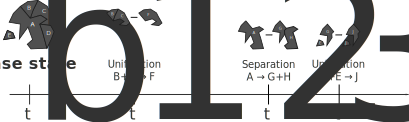
\includegraphics[width=0.8\textwidth]{graphics/basics/stdm/event-based_spatio-temporal_data_model}
%   \caption{The Event-Based Spatio-Temporal Data Model}
%   \label{fig:event-based_spatio-temporal_data_model}
% \end{figure}

history graph model without changing state: active, inactive


% ==============================================================================
\section{Hivent} % (fold)
\label{sec:hivent}

event which is in itself or whose outcome is historically significant (subjective) or with

  WHAT? significant happening
  WHO? different actors
  WHEN? one point in time
  WHERE? mostly also point in space, sometimes different from area that event affects
  WHY? because

models historically significant happenings with a focus on those who influence the geopolitical history of countries.

In modern history, geopolitical changes of countries are manifested mostly in historical treaties which are the result of a conference or any other gathering of representatives of stakeholders of that initiated change. Since each of those treaties is signed on one particular day, in one particular place and has one particular name, the ~\texttt{Hivent}~ model seems appropriate.

However, the first question arises regarding the relevance of the location: While the exact position of the battlefield of Verdun or the place where John F. Kennedy was assassinated might very relevant to the event itself, the location of a governmental bill, a declaration of independence or a border convention might not play an important role and usually happens in a representative place, e.g. the parliament or the office of a president. In a lot of cases, it is much more important which territories an event actually influences instead of where it happened.



significant happening in time and space
incluencing others
central element in event based STDM

% section hivent (end)


% ==============================================================================
\section{Area} % (fold)
\label{sec:area}

model the main entity of the domain: historical or current countries. An ~\texttt{Area}~ represents one identical country, consisting at each time point of its existance of exactly one ~\texttt{AreaName}~ and one ~\texttt{AreaTerritory}. The model seems appropriate since the name and the territory of an area are exactly the two properties that are part of the domain.

abstract: area

  defined by borders
  hierarchical structure

country borders
  coastlines
  interior
  disputed territories
    situation: n fully recognized countries and m non or partially recognized entities claim sovereignty over 1 territory
    territory is surrounded by disputed border
    question: does this disputed area claim sovereignty?
    \footnote \url{http://www.economist.com/blogs/economist-explains/2014/09/economist-explains-1}
  uncertain borders
    situation: n fully recognized countries commonly agree on a boundary between them, but the border is not clearly defined / fuzzy / uncertain
  states of borders
    planned
    agreed
    demarcated
    provisional
    valid
    vs. disputed

area
territory
-> geometry
--> border
-> representative point
name
-> short name
-> formal name

enclaves
exclaves



% section area (end)

% ==============================================================================
\section{Hivent-Based Spatio-Temporal Data Model} % (fold)
\label{sec:hivent_based_spatio_temporal_data_model}

% section hivent_based_spatio_temporal_data_model (end)


% ==============================================================================
\section{Spatio-Temporal Operations} % (fold)
\label{sec:spatio_temporal_operations}

CRE
UNI
INC
SEP
SEC
TCH
BCH
NCH
ICH
DES



inclusion of universe $\Omega$:
CRE = SEC from $\Omega$
DES = INC into $\Omega$

MECE principle: Mutually Exclusive and Collectively Exhaustive

% section spatio_temporal_operations (end)

% ==============================================================================
\section{Edit Mode} % (fold)
\label{sec:edit_mode}


user operations     CRE     UNI          SEP         TCH         NCH      DES
                     |      / \         /   \        /  \       /   \      |
HG operations       CRE   UNI   INC   SEP   SEC   TCH   BCH   NCH   ICH   DES

area changes        ADD   DEL*  DEL*  DEL   TCH   TCH   TCH   NCH   ADD   DEL
ADD, TCH, NCH, DES        ADD   TCH   ADD*  NCH?        TCH         DEL
                                NCH?        ADD*

% section edit_mode (end)

% ==============================================================================



% chapter concept (end)